\section{Customer interface}

When you are logged with a customer account in the main page you can see all the
restaurants managed by this application and all your reservations
(Figure~\ref{fig:customeriface}).

\begin{figure}[!ht]
	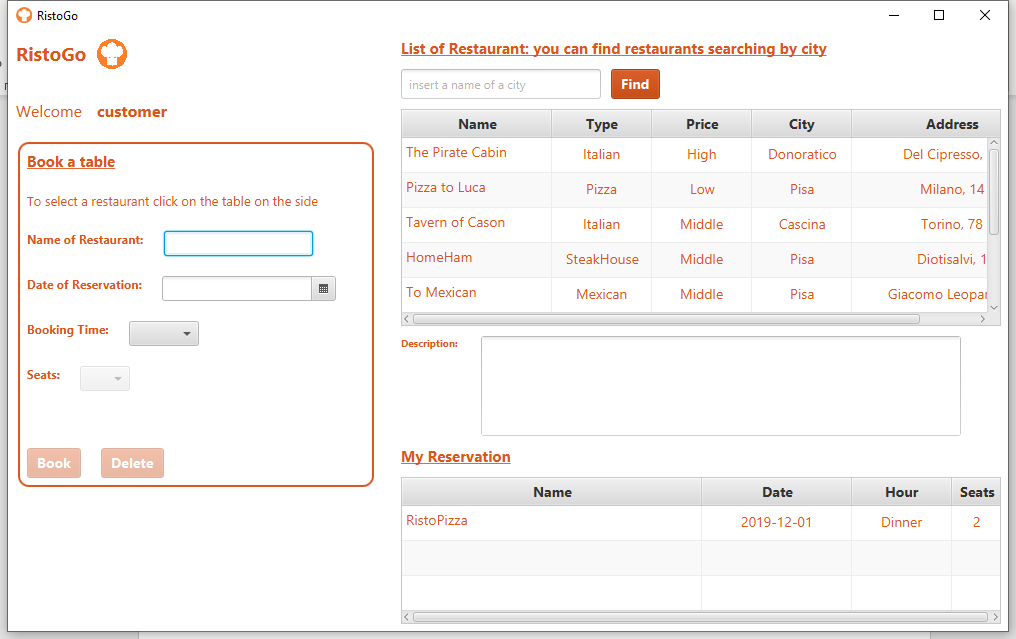
\includegraphics[width=\textwidth]{customeriface}
	\caption{Customer interface.}
	\label{fig:customeriface}
\end{figure}

\subsection{Search restaurants}

If you want to see what are the managed restaurants into a desired city, insert
the name of the city in the text field near the button ``Find'' and then click
it (Figure~\ref{fig:searchrestaurants}.

\begin{figure}[ht]
	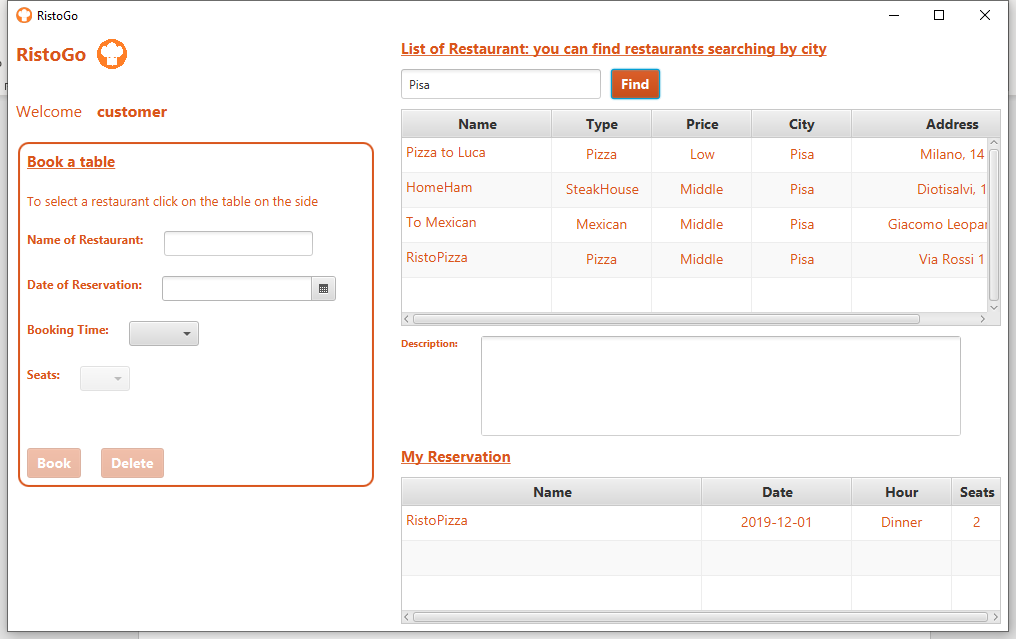
\includegraphics[width=\textwidth]{searchrestaurants}
	\caption{Search restaurants by city.}
	\label{fig:searchrestaurants}
\end{figure}

\subsection{Book a table}

To book a table, select your desired restaurant from the list. Its description
will appear in the correspondent side. Now in the section ``Book a table'' you
can find the name of the selected restaurant (Figure~\ref{fig:book}).

\begin{figure}[!ht]
	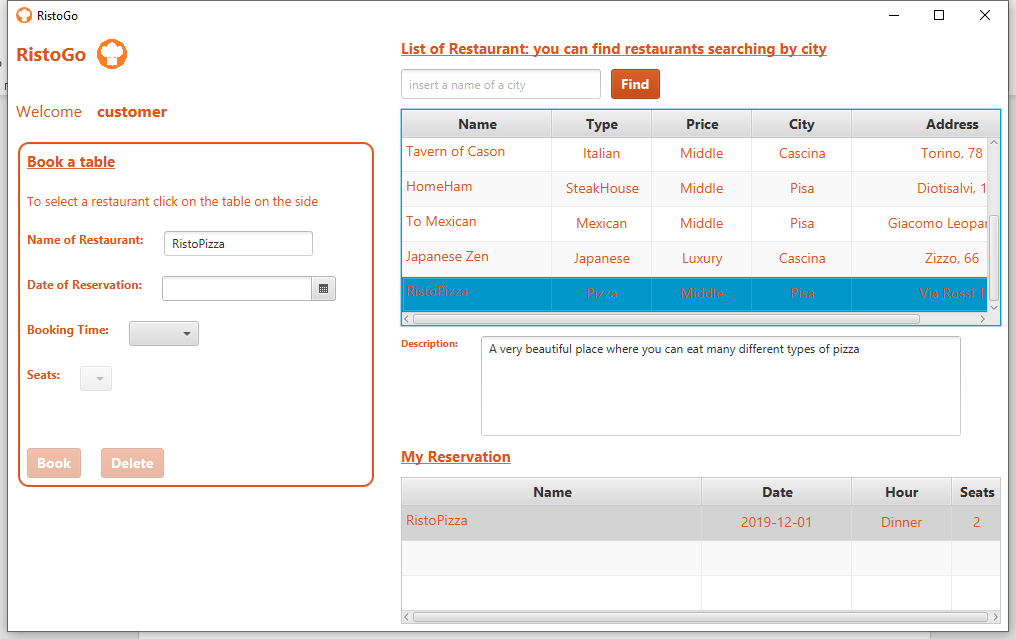
\includegraphics[width=\textwidth]{book}
	\caption{Select a restaurant to book a table.}
	\label{fig:book}
\end{figure}

Select the date, the booking time (\code{Lunch} or \code{Dinner}) and check if
there is the number of seats available that you need. If there are, select that
and click on ``Book'' to confirm (Figure~\ref{fig:completebook}).

\begin{figure}[ht]
	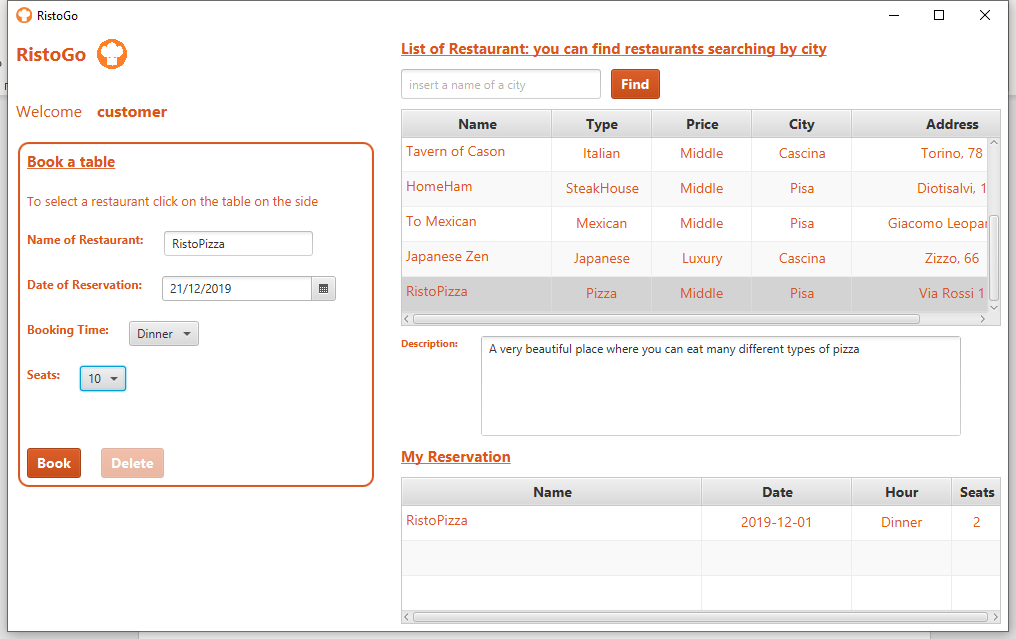
\includegraphics[width=\textwidth]{completebook}
	\caption{Fill the form to book a table.}
	\label{fig:completebook}
\end{figure}

If there are no errors, you can find your new reservation into the section ``My
Reservation'' (Figure~\ref{fig:addedreservation}).

\begin{figure}[!hb]
	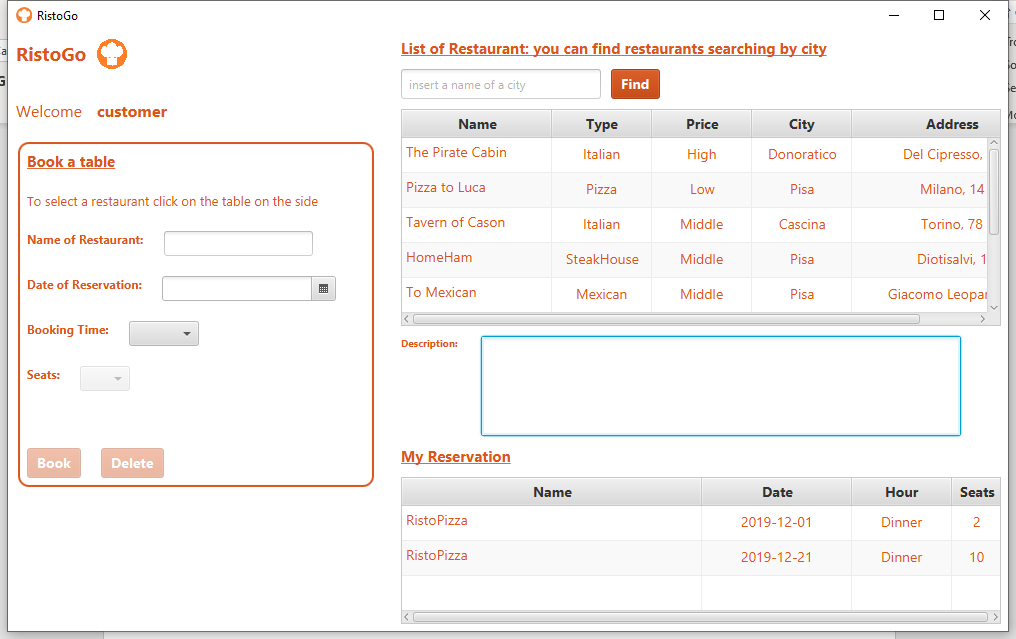
\includegraphics[width=\textwidth]{addedreservation}
	\caption{Added reservation shows in the ``My Reservation'' table.}
	\label{fig:addedreservation}
\end{figure}

\subsection{Delete a reservation}

If you want to delete a reservation, select it on the section ``My
Reservation'' (Figure~\ref{fig:deletereservation}).

\begin{figure}[ht]
	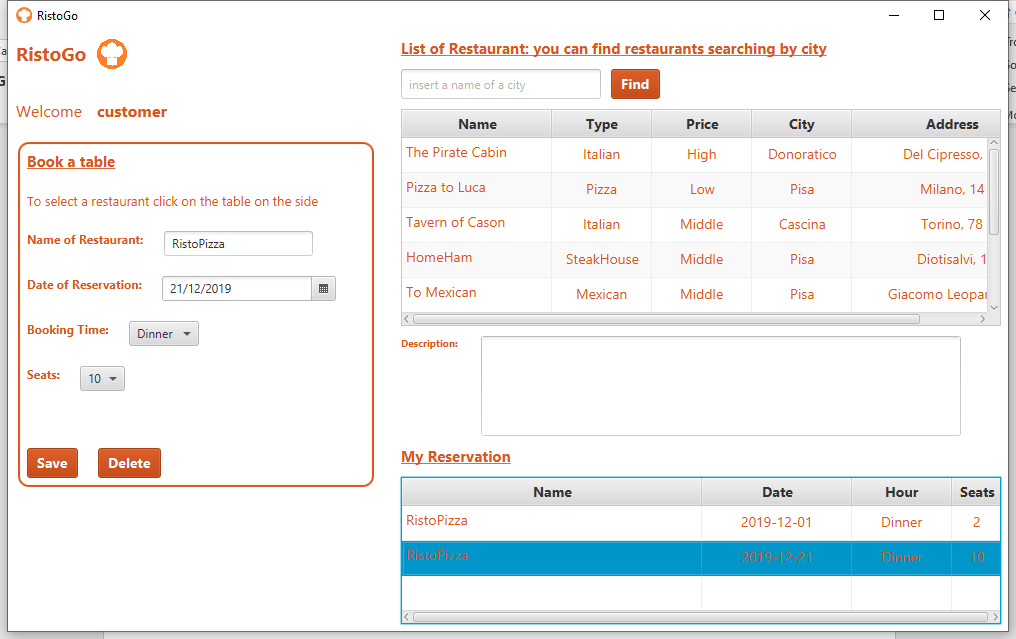
\includegraphics[width=\textwidth]{deletereservation}
	\caption{Delete a reservation.}
	\label{fig:deletereservation}
\end{figure}

Then, click on the button ``Delete'' situated on the section ``Book a table'' (for
this operation the section is empty). If there are no errors, you can see that
the reservation no longer appears in the section ``My reservation''
(Figure~\ref{fig:deletedreservation}).

\begin{figure}[!ht]
	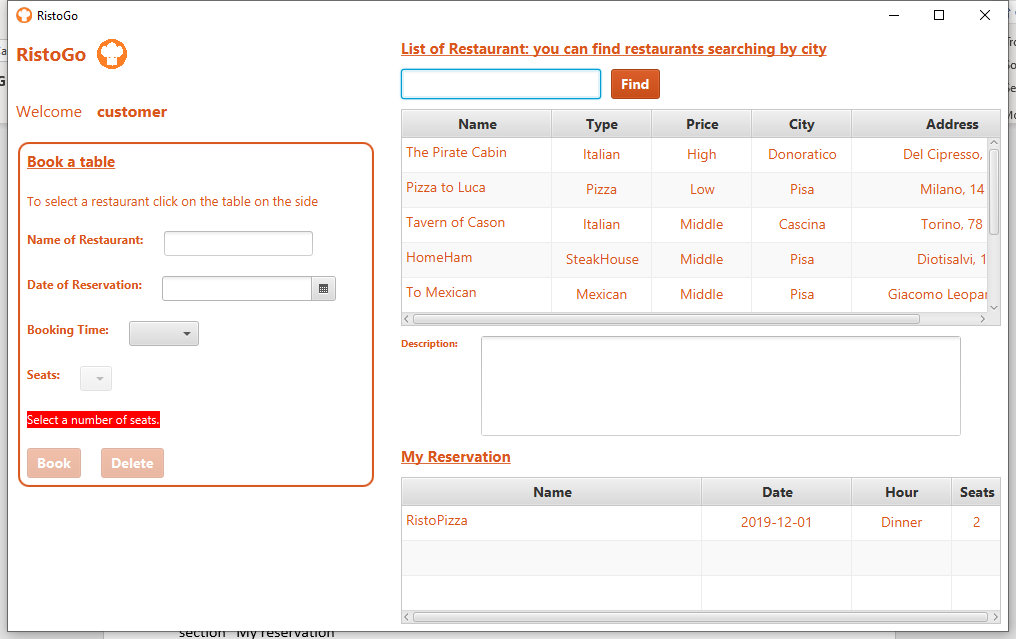
\includegraphics[width=\textwidth]{deletedreservation}
	\caption{Reservation deleted.}
	\label{fig:deletedreservation}
\end{figure}
